% ============================================================
% RAPPORT DE STAGE PFE (5A) — Douae SEBTI — INSA HdF / ALTEN
% Template : memoir (adapté du modèle de thèse UoB / V. Brena)
% Charte : bleu marine ALTEN (cohérent avec alten.fr)
% Compiler : pdflatex main.tex  (x2 pour tables et renvois)
% ============================================================
\documentclass[a4paper,11pt,leqno,openbib,oneside]{memoir}

% ---------- mise en page (héritée du template) ----------
\settrimmedsize{297mm}{210mm}{*}
\setlength{\trimtop}{0pt}
\setlength{\trimedge}{\stockwidth}
\addtolength{\trimedge}{-\paperwidth}
\settypeblocksize{634pt}{448.13pt}{*}
\setulmargins{2.7cm}{*}{*}
\setlrmargins{*}{*}{1.5}
\setmarginnotes{17pt}{51pt}{\onelineskip}
\setheadfoot{\onelineskip}{1.2\onelineskip}
\setheaderspaces{*}{1\onelineskip}{*}
\checkandfixthelayout
\frenchspacing

% ---------- encodage / langue / police ----------
\usepackage[utf8]{inputenc}
\usepackage[T1]{fontenc}
\usepackage[french]{babel}
\usepackage{lmodern}              % Latin Modern : nette et classique

\OnehalfSpacing
\setsecnumdepth{subsection}
\maxsecnumdepth{subsubsection}

% ---------- couleurs : charte ALTEN (alten.fr = bleu marine profond) ----------
\usepackage{xcolor}
\definecolor{altenink}{RGB}{20,45,70}         % bleu encre ALTEN
\definecolor{insared}{RGB}{226,0,26}          % rouge officiel INSA (blocs de chapitre)
\definecolor{altenturquoise}{RGB}{0,150,118}  % accent secondaire

% ---------- style de chapitre : sobre et professionnel ----------
% Tout en noir, aligné à gauche : « Chapitre N » puis le titre,
% un filet fin, et le mini-sommaire du chapitre (sections + sous-sections).
\usepackage{calc,soul}
\usepackage{etoc}
\makeatletter
\newcommand\chapminitoc{%
  \if@mainmatter
    \begingroup
      \etocsetnexttocdepth{subsection}%
      \etocsettocstyle{}{\vskip 4pt\hrule height 0.4pt\vskip 2pt}%
      \localtableofcontents
    \endgroup
  \fi}
\makeatother
\makechapterstyle{altenpro}{%
  \setlength{\beforechapskip}{8pt}
  \renewcommand*\chapnamefont{\normalfont\LARGE\bfseries\raggedright}
  \renewcommand*\chapnumfont{\chapnamefont}
  \renewcommand*\chaptitlefont{\normalfont\Large\bfseries\raggedright}
  \renewcommand*\afterchapternum{\par\nobreak\vskip 6pt}
  \renewcommand*\printchaptertitle[1]{\chaptitlefont ##1\par\nobreak\vskip 6pt\hrule height 1pt}
  \renewcommand*\afterchaptertitle{\vskip 16pt}
}
\chapterstyle{altenpro}

% hiérarchie des titres : chapitre (grand) > nom du chapitre (moyen) >
% section (petit) > sous-section (plus petit) > sous-sous-section (petit mais visible)
\setsecheadstyle{\large\bfseries\raggedright}
\setsubsecheadstyle{\normalsize\bfseries\raggedright}
\setsubsubsecheadstyle{\small\bfseries\raggedright}

% ---------- en-têtes : position dans le rapport à gauche, logos à droite ----------
\nouppercaseheads
\createmark{chapter}{left}{shownumber}{Chapitre~}{~---~}
\makepagestyle{altenhead}
\makeoddfoot{altenhead}{}{\thepage}{}
\makeevenfoot{altenhead}{}{\thepage}{}
\makeheadrule{altenhead}{\textwidth}{0.4pt}
\makeoddhead{altenhead}{\small\leftmark}{}%
  {
\includegraphics[height=11pt]{logo_insa.png}\enspace
\includegraphics[height=11pt]{logo_alten.png}}
\makeevenhead{altenhead}{\small\leftmark}{}%
  {
\includegraphics[height=11pt]{logo_insa.png}\enspace
\includegraphics[height=11pt]{logo_alten.png}}
\pagestyle{altenhead}
\newcommand{\clearemptydoublepage}{\newpage{\thispagestyle{empty}\clearpage}}

% ---------- paquets utiles ----------
\usepackage{graphicx}
\graphicspath{{images/}{logos/}}
\usepackage{longtable,rotating,colortbl,array,float,verbatim,enumerate,microtype}
\usepackage{amsfonts,amsmath,amssymb}
\usepackage{tikz}
\usetikzlibrary{arrows.meta,positioning,shapes,backgrounds}
\usepackage[colorlinks=true,allcolors=black]{hyperref}
\usepackage{memhfixc}

% ---------- style « mission » (hérité du rapport 4A) ----------
% chaque mission suit : Objectif -> Méthodes -> Résultats -> Discussion
\newcommand{\objectif}{\subsubsection*{a- Objectif}}
\newcommand{\methodes}{\subsubsection*{b- Méthodes utilisées}}
\newcommand{\resultats}{\subsubsection*{c- Résultats obtenus}}
\newcommand{\discussion}{\subsubsection*{d- Discussion}}
\providecommand{\ieme}{}
\renewcommand{\ieme}{\textsuperscript{ème}}

% ---------- métadonnées PDF ----------
\hypersetup{
  pdfauthor={Douae Sebti},
  pdftitle={Téléopération 5G, communication V2V et supervision d'une plateforme
            de véhicule autonome à échelle réduite sous ROS2},
}

\begin{document}

% ================= PAGE DE GARDE =================
% Page de garde — INSA Hauts-de-France / ALTEN
% Style hérité du template memoir (règles doubles), logos officiels.
\begin{titlingpage}
\begin{SingleSpace}
\calccentering{\unitlength}
\begin{adjustwidth*}{\unitlength}{-\unitlength}
\begin{center}

% ---- logos officiels ----
\begin{minipage}{0.55\textwidth}
  \centering
  
\includegraphics[width=0.9\linewidth]{logo_insa.png}
\end{minipage}\hfill
\begin{minipage}{0.35\textwidth}
  \centering
  
\includegraphics[height=3.2cm]{logo_alten.png}
\end{minipage}

\vspace{10mm}
{\large\bfseries\color{altenink} PARCOURS : 5\ieme{} année Ingénieur Mécatronique}\\[2mm]
{\large Année universitaire \textbf{2025 -- 2026}}

\vspace{12mm}
\textsc{\Large Rapport de stage PFE}\\[4mm]
\rule[0.5ex]{\linewidth}{2pt}\vspace*{-\baselineskip}\vspace*{3.2pt}
\rule[0.5ex]{\linewidth}{1pt}\\[\baselineskip]
{\huge\bfseries\color{altenink} Téléopération 5G, communication V2V et
supervision d'une plateforme de véhicule autonome à échelle réduite sous
ROS\,2}\\[4mm]
\rule[0.5ex]{\linewidth}{1pt}\vspace*{-\baselineskip}\vspace{3.2pt}
\rule[0.5ex]{\linewidth}{2pt}

\vspace{14mm}
\begin{minipage}{0.44\textwidth}
\begin{flushleft} \large
\emph{Étudiante stagiaire :}\\
Douae \textsc{Sebti}\\
{\small\itshape Stagiaire Ingénieure Mécatronique}
\end{flushleft}
\end{minipage}\hfill
\begin{minipage}{0.5\textwidth}
\begin{flushright} \large
\emph{Tuteur industriel :}\\
M. \fbox{PRÉNOM NOM} \ {\small\itshape ALTEN Labs}\\[3mm]
\emph{Tuteur pédagogique :}\\
M. Samuel \textsc{Dupont} \ {\small\itshape INSA Hauts-de-France}
\end{flushright}
\end{minipage}

\vfill
{\large ALTEN Labs --- Sèvres\\
\textsc{Institut National des Sciences Appliquées Hauts-de-France}}\\
\vspace{6mm}
\begin{minipage}{11cm}
\centering
Rapport présenté en vue de l'obtention du diplôme d'ingénieur INSA
Hauts-de-France, spécialité \textsc{Mécatronique}.
\end{minipage}\\
\vspace{8mm}
{\large\textsc{Août 2026}}
\vspace{8mm}
\end{center}
\end{adjustwidth*}
\end{SingleSpace}
\end{titlingpage}


% ================= LIMINAIRES =================
\frontmatter
\chapter*{Avant-propos}
\addcontentsline{toc}{chapter}{Avant-propos}

\section*{1- Non plagiat}
Je, soussignée \textbf{SEBTI Douae}, étudiante en Spécialité Ingénieur
Mécatronique, déclare être pleinement consciente que le plagiat d'un document ou
d'une partie de document publié sur toutes les formes existantes de support, y
compris sur Internet, constitue une violation des droits d'auteur ainsi qu'une
fraude caractérisée. En conséquence, je m'engage à citer explicitement, à chaque
fois que j'en fais usage, toutes les sources que j'ai utilisées pour écrire ce
rapport.

\vspace{0.8cm}
Fait à Sèvres, le \fbox{02/08/2026}\\
Signature\\
\textit{\underline{SEBTI Douae}}

\section*{2- Remerciements}
% TODO : à personnaliser — même esprit que ton rapport 4A :
% - ALTEN et l'équipe des Labs (tuteur industriel en premier)
% - tuteur pédagogique INSA
% - collègues du projet ProtoVA
% - tes parents (comme en 4A, c'était très beau)
\fbox{\parbox{\textwidth}{\itshape À rédiger : remerciements (tuteur industriel,
équipe ALTEN Labs, tuteur INSA, proches).}}
      % non-plagiat + remerciements
\clearpage
\tableofcontents*
\clearpage
\listoffigures
\chapter*{Glossaire}
\addcontentsline{toc}{chapter}{Glossaire}

\begin{description}
  \item[ROS 2 (Robot Operating System 2)] Intergiciel (middleware) robotique :
  les programmes sont des \emph{nœuds} qui échangent des messages sur des
  \emph{topics}. C'est l'ossature logicielle des deux ProtoVA.
  \item[DDS / FastDDS] Couche de communication de ROS 2 (découverte et échange
  de messages sur le réseau local). FastDDS est l'implémentation utilisée pour
  la téléopération WiFi.
  \item[Zenoh] Protocole de communication alternatif à DDS, adapté aux réseaux
  contraints : utilisé pour faire transiter les topics ROS 2 à travers le lien
  5G (architecture hub-and-spoke).
  \item[5G] Cinquième génération de réseaux mobiles ; ses promesses de faible
  latence et haut débit sont au c\oe ur de la téléopération de véhicules.
  \item[Téléopération] Conduite à distance du véhicule : les commandes (volant,
  vitesse) transitent par le réseau, le retour (caméra, capteurs) aussi.
  \item[V2X / V2V] \emph{Vehicle-to-Everything} / \emph{Vehicle-to-Vehicle} :
  communication directe entre véhicules pour la sécurité coopérative.
  \item[ETSI ITS] Corpus de normes européennes des systèmes de transport
  intelligents, dont les messages CAM et DENM.
  \item[CAM (Cooperative Awareness Message)] Message périodique par lequel un
  véhicule annonce sa position, son cap et sa vitesse à ses voisins.
  \item[DENM (Decentralized Environmental Notification Message)] Message
  d'alerte événementiel (ex. piéton détecté, freinage d'urgence).
  \item[Vanetza] Pile logicielle open source implémentant les normes ETSI ITS
  (GeoNetworking, CAM, DENM), embarquée sur les véhicules.
  \item[Lidar] Capteur laser rotatif mesurant les distances aux obstacles sur
  360° ; base de la cartographie et de l'évitement.
  \item[SLAM (Simultaneous Localization And Mapping)] Construction d'une carte
  de l'environnement tout en s'y localisant.
  \item[Nav2] Pile de navigation autonome de ROS 2 (planification globale et
  locale de trajectoire).
  \item[Follow the gap] Méthode de navigation réactive : chercher la plus
  grande ouverture dans le scan lidar et s'y engager.
  \item[YOLO (You Only Look Once)] Réseau de neurones de détection d'objets en
  temps réel, utilisé pour la détection de piétons.
  \item[CUDA / GPU] Calcul parallèle sur carte graphique (ici celle de la
  Jetson) pour accélérer l'inférence du réseau de neurones.
  \item[AEB (Autonomous Emergency Braking)] Freinage d'urgence automatique
  déclenché par la fusion des capteurs.
  \item[twist\_mux] Multiplexeur de commandes de vitesse ROS 2 : arbitre par
  priorité entre téléopération, navigation autonome et arrêt d'urgence.
  \item[Odométrie] Estimation du déplacement du véhicule à partir de la
  rotation de ses roues (encodeurs).
  \item[Encodeur en quadrature] Capteur délivrant deux signaux déphasés
  permettant de mesurer sens et vitesse de rotation.
  \item[Trigger de Schmitt] Circuit à hystérésis qui transforme un signal
  bruité en signal numérique propre (anti-rebond matériel).
  \item[rosbridge] Passerelle qui expose les topics ROS 2 en WebSocket/JSON,
  permettant à une page web de dialoguer avec le robot.
  \item[Jetson] Ordinateur embarqué NVIDIA avec GPU intégré, cerveau des
  véhicules ProtoVA.
\end{description}


% ================= CORPS =================
\mainmatter
\chapter*{Introduction}
\addcontentsline{toc}{chapter}{Introduction}

Mon parcours à l'INSA Hauts-de-France en spécialité Mécatronique s'achève par le
stage de fin d'études, l'ultime étape avant le métier d'ingénieure. Après une
première expérience industrielle chez FORVIA en quatrième année, où j'avais
découvert la logistique, la conception mécanique et l'outillage, je souhaitais
pour ce PFE un projet qui rassemble tout ce qui m'a menée vers la mécatronique :
la robotique, l'embarqué, les réseaux et l'automobile.

C'est exactement ce que j'ai trouvé chez \textbf{ALTEN}, au sein des
\textbf{ALTEN Labs} de Sèvres, sur le projet \textbf{ProtoVA} : une plateforme
de véhicules autonomes à échelle réduite qui sert de démonstrateur aux
technologies du véhicule connecté. Mon stage, effectué du \fbox{JJ/MM/2026} au
\fbox{JJ/MM/2026}, avait pour ambition de transformer ces prototypes en
véhicules \emph{téléopérables}, \emph{autonomes}, \emph{communicants} et
\emph{supervisables}.

% TODO : ajuster les dates, puis relire — l'intro doit annoncer le plan.
Ce rapport s'organise comme suit : je présenterai d'abord ALTEN et
l'environnement dans lequel j'ai évolué, puis je dresserai un état de l'art des
domaines abordés. Après avoir posé la problématique et la démarche, je
détaillerai mes contributions en suivant la montée en puissance du véhicule :
fiabilisation de la plateforme mécanique (Protova1), téléopération WiFi et 5G,
perception et navigation autonome, communication véhicule-à-véhicule, et enfin
supervision temps réel. Un bilan global et les perspectives clôtureront ce
travail.

\chapter{Présentation de l'entreprise}
\chapminitoc

\section{Le groupe ALTEN}

L'histoire d'ALTEN commence en 1988, lorsque trois jeunes ingénieurs issus de
grandes écoles, menés par Simon Azoulay --- toujours Président-Directeur Général
du groupe aujourd'hui ---, font un pari : les grands industriels auront de plus
en plus besoin d'externaliser une partie de leur R\&D auprès de partenaires
capables de leur fournir de l'ingénierie de haut niveau. Près de quarante ans
plus tard, ce pari est devenu le \textbf{leader mondial de l'ingénierie et des
services technologiques} (\emph{Engineering and Technology Consulting}).

Les chiffres donnent la mesure du groupe : environ \textbf{4,1 milliards
d'euros} de chiffre d'affaires en 2025, près de \textbf{58\,000 collaborateurs}
--- dont plus de \textbf{51\,000 ingénieurs et consultants} ---, une présence
dans \textbf{plus de 30 pays} et une activité réalisée aux deux tiers à
l'international. Coté à la bourse de Paris (Euronext, indice CAC Mid 60) depuis
1999, ALTEN a bâti cette croissance à la fois organiquement et par une
politique d'acquisitions soutenue en Europe, en Amérique du Nord et en Asie.

% TODO : Figure — carte d'implantation mondiale d'ALTEN (slide dispo sur
% l'intranet ou dans la plaquette « ALTEN Group Overview »)
\begin{figure}[ht]
  \centering
  \fbox{\parbox[c][4.5cm][c]{0.85\textwidth}{\centering\itshape
  Figure à insérer : implantation mondiale du groupe ALTEN\\
  (source : plaquette institutionnelle ALTEN)}}
  \caption{Présence mondiale du groupe ALTEN}
\end{figure}

\section{Secteurs d'activité}

ALTEN accompagne la R\&D des grands acteurs de pratiquement toutes les
industries de pointe : \textbf{aéronautique et spatial}, \textbf{défense et
naval}, \textbf{automobile} --- secteur historique du groupe et cadre de mon
stage ---, ferroviaire, énergie, sciences de la vie, télécommunications,
banque/finance et retail. Cette diversité est une force : les méthodes et
technologies éprouvées dans un secteur (par exemple la sûreté de
fonctionnement aéronautique) irriguent les projets des autres.

Deux grands métiers structurent l'offre : l'\textbf{ingénierie produit et
process} (conception mécanique, électronique, logiciel embarqué, essais) et les
\textbf{IT services} (systèmes d'information, données, cybersécurité). Le
véhicule autonome et connecté, à la croisée exacte de ces deux mondes ---
mécanique, embarqué, réseaux ---, est l'un des axes stratégiques de recherche
du groupe.

\section{Les ALTEN Labs}

Au-delà des projets menés chez ses clients, ALTEN investit dans sa propre
recherche à travers les \textbf{ALTEN Labs} : des structures internes agiles
dont la mission est d'explorer les technologies de rupture, de construire des
démonstrateurs concrets et de faire monter les consultants en compétence sur
les sujets d'avenir (intelligence artificielle, systèmes autonomes, 5G,
jumeaux numériques\ldots). Les Labs fonctionnent comme de petites équipes
projet pluridisciplinaires : un sujet, un encadrant, des stagiaires et
consultants, du matériel, et un objectif de démonstration.

% TODO : reprendre ici 2-3 phrases officielles de la page « Les Labs ALTEN »
% (alten.com) et citer la source en bibliographie.

\section{Le site de Sèvres}

Mon stage s'est déroulé sur le site ALTEN de \textbf{Sèvres (Hauts-de-Seine)},
au 119--121 Grande Rue, à quelques kilomètres du siège du groupe de
Boulogne-Billancourt. Ce site héberge notamment des activités de laboratoire
et les plateformes de démonstration des Labs --- dont les véhicules ProtoVA.

% TODO PHOTOS : prends 2-3 photos sur place (façade du bâtiment, l'atelier /
% la piste d'essai, les deux ProtoVA côte à côte) — bien plus percutant pour
% le jury que n'importe quelle image d'archive.
\begin{figure}[ht]
  \centering
  \fbox{\parbox[c][4.5cm][c]{0.4\textwidth}{\centering\itshape Photo à insérer :
  site ALTEN de Sèvres}}\hfill
  \fbox{\parbox[c][4.5cm][c]{0.4\textwidth}{\centering\itshape Photo à insérer :
  les véhicules ProtoVA}}
  \caption{Le site de Sèvres et la plateforme ProtoVA}
\end{figure}

\section{Le projet ProtoVA}

\textbf{ProtoVA} (\emph{Prototype de Véhicule Autonome}) est le démonstrateur
« véhicule autonome et connecté » des Labs : deux voitures à échelle réduite,
architecturées autour d'un calculateur embarqué NVIDIA Jetson et de ROS~2,
équipées d'un lidar, d'une caméra et d'une chaîne de traction instrumentée.
La plateforme sert de banc d'essai réel --- et non simulé --- aux briques du
véhicule de demain : conduite à distance via 5G, perception et navigation
autonome, communication inter-véhicules selon les normes européennes ITS, et
supervision à distance.

\begin{itemize}
  \item \textbf{Protova1} : première génération (Jetson Nano), utilisée pour
  les développements bas niveau (châssis, motorisation, odométrie) ;
  \item \textbf{Protova2} : seconde génération (Jetson Orin), qui concentre la
  téléopération, l'autonomie et la connectivité.
\end{itemize}

\section{Mon équipe et ma place dans le projet}

% TODO : organigramme (groupe -> direction Labs -> équipe ProtoVA -> toi),
% prénoms/fonctions de ton tuteur et des collègues, comme dans ton rapport 4A.
\begin{figure}[ht]
  \centering
  \fbox{\parbox[c][4cm][c]{0.85\textwidth}{\centering\itshape Figure à insérer :
  organigramme de l'équipe (encadrement ALTEN Labs et stagiaires ProtoVA)}}
  \caption{Organigramme de l'équipe d'accueil}
\end{figure}

J'ai intégré l'équipe ProtoVA en tant que stagiaire ingénieure mécatronique,
avec un périmètre volontairement transverse : mécanique (Protova1), logiciel
embarqué et réseaux (Protova2), et développement web (supervision). Cette
position m'a permis de toucher à toute la chaîne d'un véhicule autonome, du
signal d'encodeur jusqu'au message V2V --- exactement ce que je cherchais dans
ce stage de fin d'études.
   % ALTEN, Labs, Sèvres, ProtoVA
\chapter{État de l'art}
\chapminitoc
% Chapitre « niveau PFE » : montrer que tu connais le domaine AVANT de montrer
% ce que tu as fait. Chaque section : 0,5 à 1,5 page + références en biblio.

\section{Le véhicule autonome et connecté}
% TODO : niveaux d'automatisation SAE (0 à 5), architecture
% perception -> décision -> action, enjeux sécurité/société.

\section{Les middlewares robotiques : ROS 2 et DDS}
% TODO : pourquoi ROS 2 (temps réel, QoS, industrialisation), principe DDS,
% comparaison FastDDS vs Zenoh (découverte, NAT, réseaux mobiles) — ce
% comparatif justifiera tes choix du chapitre 5.

\section{La téléopération de véhicules et l'apport de la 5G}
% TODO : exigences de latence pour la conduite à distance (~<100 ms),
% architectures 5G (NSA/SA), cas d'usage industriels existants.

\section{Les communications V2X}
% TODO : ITS-G5 (802.11p) vs C-V2X ; normes ETSI : CAM (EN 302 637-2),
% DENM (EN 302 637-3), GeoNetworking ; piles logicielles dont Vanetza.
% C'est le socle théorique de TON chapitre 7.

\section{Perception embarquée}
% TODO : lidar 2D, détection par apprentissage profond (famille YOLO),
% fusion capteurs, principe de l'AEB.

\section{Localisation et navigation autonome}
% TODO : SLAM (slam_toolbox), pile Nav2, méthodes réactives (follow the gap,
% issue de la compétition F1TENTH).

\section{Les plateformes à échelle réduite}
% TODO : F1TENTH, Duckietown, etc. : pourquoi la recherche utilise des
% voitures 1/10 — coût, sécurité, itération rapide. Positionner ProtoVA.

\section{Synthèse : les verrous adressés par ce stage}
% TODO : 4-5 verrous concrets qui font la transition vers le chapitre 3
% (ex. « la latence 5G est-elle compatible avec la téléopération ? »,
% « les piles ETSI sont-elles utilisables sans matériel 802.11p dédié ? »).
     % État de l'art
\chapter{Contexte, problématique et démarche}
\chapminitoc

\section{Contexte : l'existant à mon arrivée}
% TODO : état des deux véhicules à ton arrivée (ce qui marchait, ce qui
% manquait), comme le « Contexte » de tes chapitres 4A.

\section{Problématique}
% La question unique qui chapeaute tout le rapport — encadrée, bien visible.
\begin{center}
\fbox{\parbox{0.9\textwidth}{\itshape
Comment transformer des prototypes de véhicules à échelle réduite en une
plateforme téléopérable, autonome et communicante --- fiable du niveau
mécanique jusqu'au niveau applicatif --- tout en instrumentant ses performances
réseau (WiFi/5G) pour en démontrer la viabilité ?}}
\end{center}
% TODO : reformule-la avec tes mots, puis décline-la en sous-questions.

\section{Objectifs et cahier des charges}
% TODO : tableau objectifs / livrables / critères de réussite
% (téléop 5G opérationnelle, V2V CAM+DENM démontré, base Protova1 fiabilisée,
% dashboard fonctionnel, etc.)

\section{Démarche et planning}
% TODO : Gantt prévisionnel vs réalisé (figure), méthode de travail
% (itérations, démos régulières).

\section{Moyens mis à disposition}
% TODO : matériel (Jetson, RPLIDAR A1, caméra Orbbec, dongle 5G, volant G29,
% imprimante 3D...) et logiciels (ROS 2 Humble, Inventor/CAO, Vanetza...).

\section{Organisation et communication}
% TODO : rituels d'équipe, échanges avec les tuteurs (CDC envoyé, bilans
% intermédiaires) — la grille INSA note explicitement ce point.
     % Contexte, problématique, démarche
\chapter{Fiabilisation de la plateforme Protova1 : mécanique et odométrie}

\section{Contexte}
% TODO : Protova1, première génération : base mécanique vieillissante,
% odométrie inexploitable à cause des rebonds de l'encodeur.

\section{Problématique}
% TODO : comment redonner à Protova1 une base saine (mécanique + mesure de
% déplacement fiable) pour en faire à terme un second véhicule téléopérable ?

\section{Mission 1 : Conception et impression 3D de la nouvelle base mécanique}
\objectif
% TODO : remplacer la base existante ; contraintes d'intégration (fixations
% Jetson/lidar/batterie, rigidité, masse).
\methodes
% TODO : CAO (mêmes réflexes que tes conceptions FORVIA : cahier des charges,
% itérations de solutions, choix justifié), impression 3D : matériau,
% orientation, tolérances, assemblage.
\resultats
% TODO : photos avant/après, masse, qualité d'assemblage.
\discussion
% TODO : itérations ratées/réussies, leçons (tolérances d'impression...).

\section{Mission 2 : Chaîne odométrique --- filtrage de l'encodeur}
\objectif
% TODO : signaux du KY-040 inexploitables (rebonds) -> compter proprement les
% ticks pour l'odométrie.
\methodes
% TODO : analyse du signal brut, conception du conditionnement : filtre RC +
% trigger de Schmitt 74HC14, schéma électronique, dimensionnement justifié
% (choix R, C, seuils d'hystérésis), banc de test Arduino en quadrature.
\resultats
% TODO : LE chiffre : 1 tour = 80 ticks, stable et reproductible — mets
% l'oscillogramme avant/après filtrage, c'est très parlant.
\discussion
% TODO : limites (résolution, vitesse max), alternative logicielle écartée.

\section{Vers la téléopération de Protova1}
% TODO : perspective — ce qui reste à faire pour rendre Protova1 téléopérable
% comme Protova2 (annonce des perspectives de la conclusion générale).

\section{Conclusion}
% TODO : 4-5 lignes de bilan du chapitre.
     % Mécanique + odométrie Protova1
\chapter{Téléopération de Protova2 : WiFi et 5G}
\chapminitoc
\label{chap:teleop}

\section{Contexte}

Avant de rendre un véhicule autonome, il faut pouvoir le conduire à distance :
la téléopération est à la fois un mode d'exploitation à part entière (conduite
déportée avec retour vidéo), un outil de développement indispensable
(cartographie manuelle pour le SLAM, essais de perception) et le mode de repli
de sécurité lorsque l'autonomie est en défaut. Sur Protova2, le poste de
pilotage est un PC équipé d'un volant à retour de force Logitech G29 ; le
véhicule embarque la Jetson Orin Nano, qui pilote les actionneurs via le
microcontrôleur Pico et renvoie le flux de sa caméra.

J'ai mis en œuvre et comparé deux liaisons radio pour cette téléopération : le
\textbf{WiFi} du laboratoire, puis un \textbf{réseau 5G privé}, représentatif
des déploiements industriels visés pour les véhicules connectés.

\section{Problématique}

La téléopération est une \emph{boucle} : l'opérateur perçoit la scène à
travers la vidéo, agit sur le volant, et sa commande traverse le réseau avant
d'atteindre les roues. Ce que voit l'opérateur est donc toujours \emph{le
passé} du véhicule, et sa commande arrive toujours \emph{en retard} sur ce
qu'il a vu. La qualité de conduite dépend ainsi de trois grandeurs : la
\textbf{latence} (le retard de la boucle), le \textbf{débit} (la capacité à
transporter la vidéo) et la \textbf{cadence d'images} (la fluidité du retour
visuel). L'un des enjeux du chapitre est précisément de déterminer laquelle de
ces grandeurs est réellement dimensionnante.

À cette problématique de performance s'ajoute une problématique
d'intégration : le middleware de ROS~2 (DDS) repose sur la découverte
\emph{multicast}, qui fonctionne nativement sur un réseau local WiFi mais
\textbf{ne traverse pas un réseau cellulaire}. La liaison 5G impose donc une
architecture de transport différente de celle du WiFi.

\section{Architecture logicielle de commande}

La chaîne de commande est identique quel que soit le support radio ; seul le
transport change. Côté PC, \texttt{joy\_node} lit le volant et publie
\texttt{/joy} ; côté véhicule, \texttt{g29\_teleop} convertit ces axes en
consigne de conduite (\texttt{/cmd\_vel\_G29}), un multiplexeur
(\texttt{twist\_mux}) arbitre entre les sources de commande par priorité ---
la téléopération, la navigation autonome et le freinage d'urgence (priorité
maximale, chapitre~\ref{chap:perception}) --- et le nœud série \texttt{TX}
transmet la consigne retenue au Pico, qui commande le servomoteur de direction
et le variateur de traction. En sens inverse, la caméra Orbbec publie son flux
couleur compressé JPEG, visualisé sur le PC. Chaque entrée du multiplexeur est
assortie d'un \emph{timeout} : une source qui cesse d'émettre perd la main,
ce qui garantit qu'une coupure réseau conduit à l'arrêt et non à la poursuite
de la dernière commande reçue.

\begin{figure}[ht]
  \centering
  \begin{tikzpicture}[x=1mm, y=1mm,
      boite/.style={draw=altenink, fill=altenink!8, rounded corners=2pt,
                    minimum height=8mm, minimum width=22mm, align=center, font=\small},
      lien/.style={-{Stealth[length=2.5mm]}, thick, color=black!55},
      etiq/.style={font=\tiny\ttfamily, color=black!55}]
    \node[boite] (joy)  at (0,0)    {volant G29\\+ \texttt{joy\_node} (PC)};
    \node[boite] (g29)  at (40,0)   {\texttt{g29\_teleop}};
    \node[boite] (mux)  at (76,0)   {\texttt{twist\_mux}\\(priorités)};
    \node[boite] (tx)   at (110,0)  {\texttt{TX} série};
    \node[boite] (pico) at (141,0)  {Pico\\servo + ESC};
    \node[boite] (cam)  at (76,-22) {caméra Orbbec\\(JPEG 720p)};
    \node[boite] (pcv)  at (20,-22) {visualisation\\PC};
    \draw[lien] (joy.east)  -- node[etiq, above]{/joy \ (réseau)} (g29.west);
    \draw[lien] (g29.east)  -- node[etiq, above]{/cmd\_vel\_G29} (mux.west);
    \draw[lien] (mux.east)  -- node[etiq, above]{/cmd\_vel} (tx.west);
    \draw[lien] (tx.east)   -- node[etiq, above]{série} (pico.west);
    \draw[lien] (cam.west)  -- node[etiq, above]{images \ (réseau)} (pcv.east);
  \end{tikzpicture}
  \caption{Chaîne de téléopération : les commandes descendent du PC vers le
  véhicule, la vidéo remonte. Les liens marqués « réseau » traversent le WiFi
  ou la 5G selon la configuration.}
  \label{fig:chaine-teleop}
\end{figure}

\section{Mission 1 : Téléopération WiFi (FastDDS)}

\objectif
Conduire Protova2 au volant G29 à travers le WiFi du laboratoire, avec retour
vidéo temps réel, en utilisant le transport natif de ROS~2.

\methodes
Sur un réseau local, le DDS natif de ROS~2 (FastDDS) suffit : les deux
machines partagent le même domaine (\texttt{ROS\_DOMAIN\_ID=125}) et la
découverte multicast fait le reste, sans configuration supplémentaire. J'ai
encapsulé le lancement dans des scripts symétriques
(\texttt{launch\_pc\_wifi.sh} côté poste, \texttt{launch\_car\_wifi.sh} côté
véhicule) qui fixent l'environnement, nettoient les instances précédentes et
démarrent les nœuds dans l'ordre. Un point de vigilance : les flux d'images
doivent être publiés et souscrits en QoS \emph{best-effort} --- en mode
\emph{reliable}, les retransmissions DDS s'accumulent sur un lien radio et le
flux se fige.

\resultats
La conduite au volant fonctionne avec un retour vidéo fluide. La
caractérisation du lien (protocole détaillé en
section~\ref{sec:campagne-mesures}) donne : latence moyenne de \textbf{68~ms}
mais très irrégulière (pointes à 237~ms), débit d'environ \textbf{185~Mbps}
dans les deux sens, et cadence vidéo de \textbf{30~images/s} --- la pleine
cadence de la caméra.

\discussion
Le débit WiFi est très confortable, mais la latence présente une particularité
contre-intuitive que mes mesures ont mise en évidence : elle est \emph{pire à
vide qu'en charge} (84~ms au repos contre 59~ms sous trafic soutenu). Il
s'agit de l'économie d'énergie de la radio WiFi : entre deux paquets, elle
s'endort, et son réveil coûte 100 à 300~ms. Ce comportement, sans conséquence
pour de la bureautique, est pénalisant pour une boucle de pilotage, où les
commandes sont justement de petits paquets épars.

\section{Mission 2 : Téléopération 5G (Zenoh)}

\objectif
Reproduire la téléopération complète à travers un réseau 5G privé, en
remplaçant le transport DDS, inopérant sur un lien cellulaire.

\methodes
Chaque machine est équipée d'un modem 5G Quectel (RM520N côté PC, RM530N côté
véhicule). Le multicast étant impossible sur ce lien, j'ai remplacé le
transport par \textbf{Zenoh} (\texttt{rmw\_zenoh\_cpp}) en architecture
\emph{hub-and-spoke} : un routeur Zenoh sur le PC écoute sur le port 7447 ; le
routeur du véhicule ouvre une connexion TCP vers lui à travers la 5G ; et les
nœuds ROS~2 de chaque machine se connectent en clients à leur routeur local.
Deux subtilités de configuration méritent d'être notées : \texttt{rmw\_zenoh}
ignore la variable \texttt{ZENOH\_CONFIG} et exige
\texttt{ZENOH\_ROUTER\_CONFIG\_URI} / \texttt{ZENOH\_SESSION\_CONFIG\_URI} ;
et les sessions des nœuds ne se rattachent pas à un routeur redémarré, ce qui
impose un ordre de démarrage strict.

\resultats
La chaîne complète fonctionne à travers la 5G : appairage des routeurs vérifié
(session TCP établie sur le port 7447 à travers le lien radio), commandes du
volant reçues par le véhicule, vidéo remontée au poste. Les performances
mesurées figurent en section~\ref{sec:campagne-mesures}.

\discussion
Le débogage le plus instructif a concerné l'\textbf{adressage IP}. Les
symptômes : le lien 5G semblait mort --- \texttt{ping 172.16.48.7} répondait
\emph{« Do you want to ping broadcast? »} --- alors que la radio était
parfaitement fonctionnelle. Le diagnostic : le modem attribue par DHCP une
adresse en \texttt{/30}, un sous-réseau de quatre adresses seulement, dans
lequel \texttt{.7} --- précisément l'adresse du poste de pilotage --- est
l'\emph{adresse de diffusion} : le noyau refuse alors tout trafic unicast vers
le PC. La correction consiste à élargir le masque en \texttt{/28}
(\texttt{.7} redevient une adresse d'hôte ordinaire) et à purger
systématiquement la \texttt{/30} que chaque renouvellement de bail DHCP
réintroduit.

Plus généralement, aucune des difficultés rencontrées n'incombait au protocole
Zenoh lui-même : toutes relevaient de l'\emph{intégration système} ---
installation, variables d'environnement, adressage, ordonnancement du
démarrage, et jusqu'à ce piège d'exploitation : un \texttt{pkill}
lancé à travers SSH avec le nom d'un nœud en argument peut tuer sa propre
session, le motif se retrouvant dans la ligne de commande du shell distant.
La méthode qui a permis d'en venir à bout est la vérification \emph{maillon
par maillon} : interface $\rightarrow$ adresse IP $\rightarrow$ \texttt{ping}
$\rightarrow$ session TCP 7447 $\rightarrow$ graphe ROS. Enfin, pour rendre
l'ensemble robuste aux aléas, j'ai confié la pile du véhicule à un service
\textbf{systemd} (\texttt{car5g.service}) : elle démarre au boot, se relance
seule en cas d'échec et ne dépend plus d'aucun terminal ouvert.

\section{Campagne de mesures : WiFi vs 5G}
\label{sec:campagne-mesures}

\objectif
Comparer objectivement les deux liaisons sur les trois grandeurs de la
téléopération --- latence, débit, cadence vidéo --- avec des outils
reproductibles.

\methodes
J'ai développé trois scripts de mesure autonomes, chacun produisant sa courbe
et ses données brutes : \texttt{mesure\_latence.py} (RTT de chaque paquet
\texttt{ping}, 5~Hz), \texttt{mesure\_debit.py} (débit utile transféré chaque
seconde par \texttt{iperf3}, dans les deux sens) et \texttt{mesure\_fps.py}
(comptage, seconde par seconde, des images reçues au poste de pilotage). Les
mêmes scripts servent pour les deux réseaux --- seule change la cible --- ce
qui garantit une comparaison à protocole identique. Ils complètent les
tableaux de bord de supervision en direct présentés au
chapitre~\ref{chap:dashboard}.

\resultats
La figure~\ref{fig:comparaison-wifi-5g} superpose les mesures ; le
tableau~\ref{tab:wifi-5g} les résume.

\begin{figure}[ht]
  \centering
  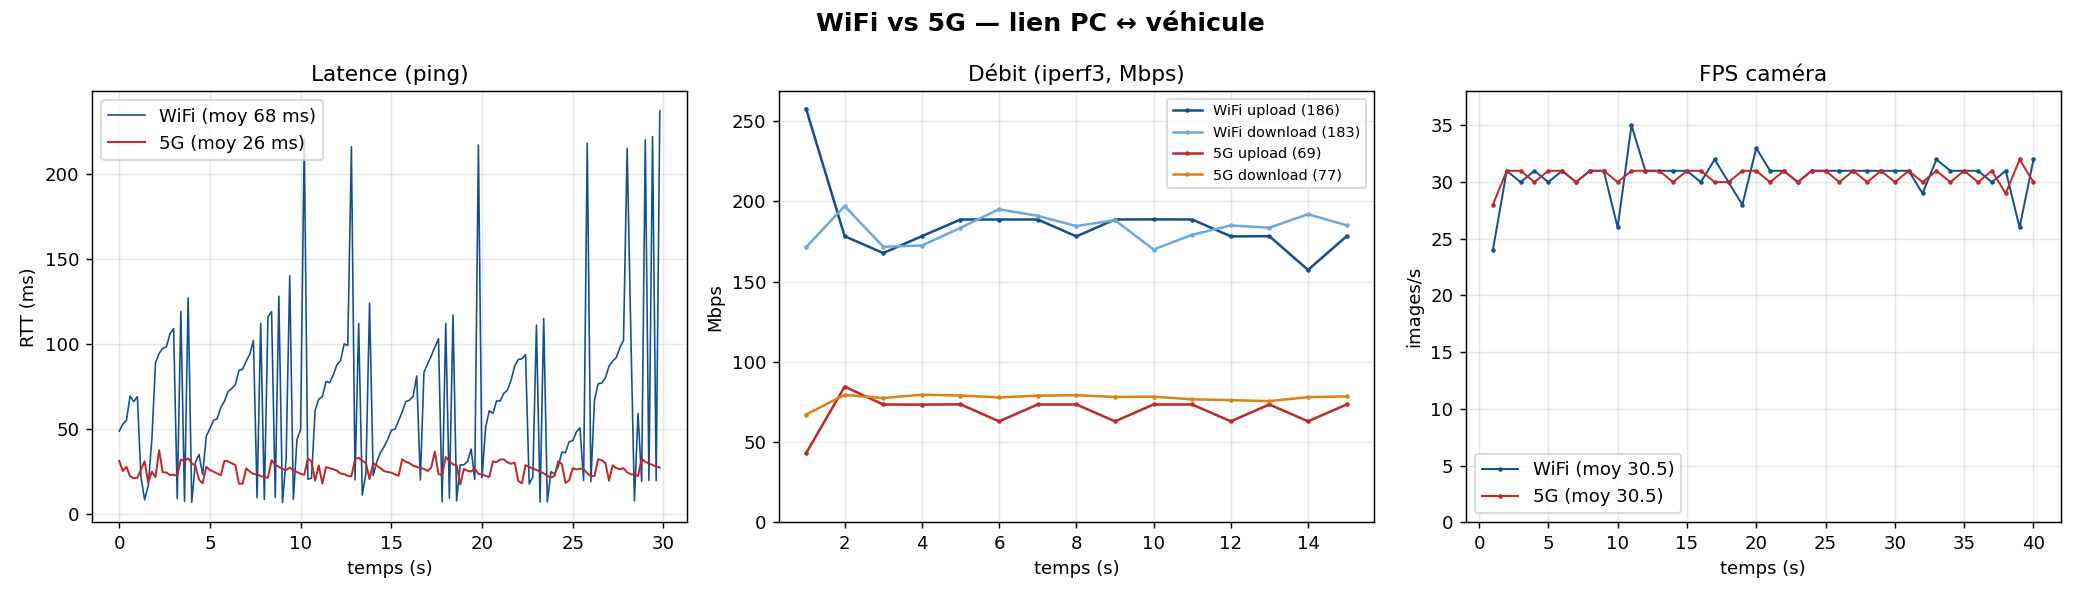
\includegraphics[width=\textwidth]{comparaison_wifi_5g.png}
  \caption{Comparaison WiFi / 5G sur le lien PC $\leftrightarrow$ véhicule :
  latence (gauche), débit dans les deux sens (centre), cadence vidéo
  (droite).}
  \label{fig:comparaison-wifi-5g}
\end{figure}

\begin{table}[ht]
  \centering
  \begin{tabular}{lccc}
    \hline
    \textbf{Grandeur} & \textbf{WiFi} & \textbf{5G} & \textbf{Écart} \\
    \hline
    Latence moyenne (gigue)          & 68 ms (pointes 237)  & \textbf{26 ms} (17--37) & 5G $\times$2,6 \\
    Débit montant PC$\to$véhicule    & \textbf{186 Mbps}    & 69 Mbps   & WiFi $\times$2,7 \\
    Débit descendant véhicule$\to$PC & \textbf{183 Mbps}    & 77 Mbps   & WiFi $\times$2,4 \\
    Cadence vidéo 720p               & 30,5 im/s            & 30,5 im/s & égalité \\
    \hline
  \end{tabular}
  \caption{Synthèse des mesures WiFi / 5G (moyennes des campagnes).}
  \label{tab:wifi-5g}
\end{table}

\discussion
Ces résultats illustrent une distinction essentielle : le débit et la cadence
d'images sont des critères \emph{à seuil}, tandis que la latence est le
\emph{facteur de mérite}. Le besoin réel du système est modeste --- environ
18~Mbps pour la vidéo 720p, moins de 0,1~Mbps pour les commandes --- et les
deux liens le dépassent largement : la vidéo passe d'ailleurs à pleine cadence
(30~im/s) sur les deux. L'avantage de débit du WiFi ne se traduit donc par
aucun bénéfice perceptible. La latence, en revanche, intervient dans la boucle
perception--action à chaque instant et ne peut être compensée par aucun autre
paramètre : à 1~m/s, les 68~ms moyens du WiFi (et surtout ses pointes à
237~ms) représentent 7 à 24~cm parcourus « à l'insu » de l'opérateur, contre
moins de 3~cm --- et de façon \emph{prévisible} --- en 5G. Pour la
téléopération temps réel, la 5G est donc le lien le plus adapté, par sa
latence faible et \emph{stable} bien plus que par toute autre caractéristique.

Une perspective naturelle est la \textbf{mobilité} : le \emph{handover}
(changement de point d'accès en mouvement) est natif et quasi transparent en
5G --- c'est l'un de ses atouts fondateurs pour le véhicule connecté ---
tandis que le \emph{roaming} WiFi, décidé par le client, provoque des coupures
de quelques centaines de millisecondes à plusieurs secondes. Le bâtiment du
laboratoire, couvert par une vingtaine de bornes WiFi, se prête à une mesure
comparative de ces interruptions, qui constituerait un prolongement direct de
cette campagne.

\section{Conclusion}

La téléopération de Protova2 fonctionne de bout en bout sur les deux liaisons,
avec une chaîne de commande commune et deux transports adaptés à chaque
support (FastDDS en WiFi, Zenoh en hub-and-spoke sur 5G). La campagne de
mesures, menée avec des outils développés pour être reproductibles, dégage la
conclusion structurante du chapitre : à débit suffisant --- ce qui est le cas
des deux liens --- c'est la latence, et sa stabilité, qui gouverne la qualité
de la téléopération ; la 5G y est nettement supérieure (26~ms stables contre
68~ms irréguliers). Ce résultat, ainsi que la robustesse apportée par la
supervision systemd de la pile embarquée, préparent le terrain du
chapitre~\ref{chap:v2v}, où le lien inter-véhicules transporte non plus des
commandes de conduite mais des messages de sécurité coopérative.
       % Téléopération WiFi / 5G — RÉDIGÉ
\chapter{Perception et navigation autonome}
\label{chap:perception}

\section{Contexte}
% TODO : après la téléopération, rendre le véhicule capable de « voir » et de
% décider seul — et fournir la perception qui alimentera le V2V (chap. 7).

\section{Problématique}
% TODO : percevoir (lidar + caméra), se localiser, naviguer et freiner seul,
% avec les ressources limitées d'un calculateur embarqué.

\section{Mission 1 : Cartographie et localisation (SLAM)}
\objectif
\methodes
% TODO : RPLIDAR -> slam_toolbox, réglages, cartes obtenues.
\resultats
\discussion

\section{Mission 2 : Navigation réactive follow the gap et avancement Nav2}
\objectif
\methodes
% TODO : principe follow_the_gap sur le scan lidar, package navigation,
% intégration twist_mux (priorités avec la téléop) ; état d'avancement Nav2.
\resultats
\discussion

\section{Mission 3 : Détection de piétons par vision --- YOLO embarqué sur GPU}
\objectif
\methodes
% TODO : portage de l'inférence sur le GPU de la Jetson : JetPack/CUDA,
% installation de torch spécifique Jetson, numpy compatible — le chemin de
% croix technique mérite d'être raconté.
\resultats
% TODO : LE tableau avant/après : 344 ms/image (CPU) -> 30 ms/image (GPU),
% soit un facteur ~11 — ton meilleur résultat chiffré du chapitre.
\discussion

\section{Mission 4 : Freinage d'urgence automatique (AEB) par fusion lidar + caméra}
\objectif
\methodes
% TODO : fusion aeb_fusion (offset 180° du lidar, seuils dynamiques selon la
% vitesse, frein actif calibré, timeout twist_mux), « boîte noire » de debug.
\resultats
% TODO : scénarios d'essai (obstacle statique, piéton), distances d'arrêt.
\discussion

\section{Conclusion}
   % SLAM, YOLO, AEB
\chapter{Communication véhicule-à-véhicule (V2V)}
\label{chap:v2v}
% ⭐ TON chapitre vedette : contribution conçue et réalisée de bout en bout
% par toi, from scratch. Rédige-le en « j'ai choisi / j'ai conçu / j'ai
% démontré ».

\section{Contexte}
% TODO : pour la sécurité coopérative, les véhicules doivent s'annoncer
% mutuellement (CAM) et s'alerter (DENM) — normes ETSI vues au chapitre 2.

\section{Problématique}
% TODO : implémenter une communication V2V conforme ETSI sur du matériel
% standard (WiFi, sans carte 802.11p dédiée), intégrée à ROS 2, et la
% démontrer entre deux véhicules réels.

\section{Mission 1 : Mise en \oe uvre de la pile Vanetza embarquée}
\objectif
\methodes
% TODO : choix de Vanetza (comparaison avec les alternatives), compilation
% croisée/embarquée avec backend OpenSSL, socktap sur interface WiFi.
\resultats
\discussion

\section{Mission 2 : Émission et réception de CAM intégrées à ROS 2}
\objectif
\methodes
% TODO : v2v_node — contenu des CAM, fréquence, topics /v2v/remote_vehicles,
% /v2v/alert ; stratégies de positionnement (GPS simulé, odométrie, distance
% lidar réelle via lidar_neighbor).
\resultats
% TODO : captures des CAM reçus, portée, fréquence effective.
\discussion

\section{Mission 3 : Alertes DENM déclenchées par la perception}
\objectif
\methodes
% TODO : chaînage perception (chap. 6) -> DENM : détection piéton YOLO
% (/obstacle/detections) -> émission DENM -> réaction du véhicule récepteur.
\resultats
% TODO : LA démo à deux véhicules : scénario, mesures, captures d'écran.
\discussion

\section{Conclusion}
          % Vanetza CAM / DENM (chapitre vedette)
\chapter{Supervision temps réel : dashboard de télémétrie}
\label{chap:dashboard}

\section{Contexte}
% TODO : besoin d'un poste de supervision unique : état du véhicule, carte,
% lidar, latence réseau, messages V2V — visibles dans un simple navigateur.

\section{Problématique}
% TODO : exposer les données ROS 2 du véhicule à une interface web, en temps
% réel, à travers WiFi comme 5G, sans saturer le lien.

\section{Mission : Conception et développement du dashboard web}
\objectif
% TODO : spécifications des panneaux (carte SLAM, lidar, vitesse, latence
% WiFi/5G superposées, feed CAM/DENM).
\methodes
% TODO : architecture rosbridge (WebSocket :9090) + React/TypeScript +
% roslib ; nœud telemetry_bridge côté Jetson (ping, température CPU, mode
% wifi/5g) ; throttling des topics pour préserver la bande passante ;
% piège du ROS_DOMAIN_ID raconté en discussion.
\resultats
% TODO : captures d'écran du dashboard en fonctionnement (lidar live,
% courbes WiFi vs 5G superposées) ; usage pendant les démos.
\discussion
% TODO : choix React vs Foxglove justifié ; limites et évolutions (caméra,
% TF map->odom pour la pose exacte).

\section{Conclusion}
    % Dashboard de supervision
\chapter{Bilan général du projet}
\chapminitoc
% Ce chapitre est rare dans les rapports étudiants et c'est PRÉCISÉMENT ce
% que la grille INSA note : valeur ajoutée, facteur humain, synthèse.

\section{Synthèse des résultats au regard des objectifs}
% TODO : tableau objectifs (chap. 3) vs résultats obtenus vs statut ✓/partiel,
% avec renvoi aux chapitres.

\section{Valeur ajoutée pour ALTEN}
% TODO : plateforme de démonstration opérationnelle (démos clients/salons),
% documentation et scripts laissés (reproductibilité), briques réutilisables
% (V2V, dashboard), montée en maturité du Lab sur la 5G et l'ITS.

\section{Facteur humain et travail d'équipe}
% TODO : collaboration dans l'équipe ProtoVA, passation aux prochains
% stagiaires, communication avec les tuteurs (CDC, bilans), démos publiques.

\section{Compétences développées}
% TODO : techniques (ROS 2, réseaux 5G, normes ETSI, CAO/3D, électronique,
% web) et transverses (gestion de projet, autonomie, vulgarisation).
        % Bilan général du projet
\chapter*{Conclusion générale et perspectives}
\addcontentsline{toc}{chapter}{Conclusion générale et perspectives}

% TODO : même esprit que ta conclusion 4A (sincère, personnelle) mais niveau
% PFE : rappel de la problématique -> réponse apportée -> perspectives
% techniques -> bilan personnel et professionnel.
%
% Perspectives à développer :
%  - rendre Protova1 téléopérable à son tour (base fiabilisée au chap. 4) ;
%  - perception coopérative : fusionner les CAM reçus avec le lidar pour la
%    prédiction de collision (suite naturelle du chap. 7) ;
%  - navigation Nav2 complète ;
%  - dashboard : flux caméra et pose TF exacte.

\fbox{\parbox{\textwidth}{\itshape Conclusion à rédiger en dernier, une fois
tous les chapitres stabilisés.}}


% ================= BIBLIO + ANNEXES =================
\begin{thebibliography}{99}
\addcontentsline{toc}{chapter}{Bibliographie}

\bibitem{alten} ALTEN Group, \emph{Site institutionnel et résultats annuels},
\url{https://www.alten.com} --- consulté en 2026.

\bibitem{altenlabs} ALTEN Group, \emph{Les Labs ALTEN : un temps d'avance sur
l'innovation}, \url{https://www.alten.com/fr/les-labs-alten-un-temps-davance-sur-linnovation/}.

\bibitem{sae} SAE International, \emph{J3016 : Taxonomy and Definitions for
Terms Related to Driving Automation Systems}, 2021.

\bibitem{ros2} Open Robotics, \emph{ROS 2 Documentation (Humble)},
\url{https://docs.ros.org}.

\bibitem{etsi-cam} ETSI, \emph{EN 302 637-2 : Intelligent Transport Systems ;
Cooperative Awareness Basic Service (CAM)}.

\bibitem{etsi-denm} ETSI, \emph{EN 302 637-3 : Intelligent Transport Systems ;
Decentralized Environmental Notification Basic Service (DENM)}.

\bibitem{vanetza} R. Riebl et al., \emph{Vanetza : an open-source
implementation of the ETSI ITS protocol stack},
\url{https://www.vanetza.org}.

\bibitem{zenoh} Eclipse Foundation, \emph{Zenoh : Zero Overhead Network
Protocol}, \url{https://zenoh.io}.

\bibitem{f1tenth} M. O'Kelly et al., \emph{F1TENTH : An Open-source Evaluation
Environment for Continuous Control and Reinforcement Learning}, NeurIPS 2019.

\bibitem{yolo} J. Redmon et al., \emph{You Only Look Once : Unified, Real-Time
Object Detection}, CVPR 2016.

\bibitem{nav2} S. Macenski et al., \emph{The Marathon 2 : A Navigation System},
IROS 2020.

% TODO : compléter au fil de la rédaction (3GPP 5G, slam_toolbox, articles
% téléopération...) — la grille INSA valorise une biblio réelle et citée
% dans le texte via \cite{...}.
\end{thebibliography}

\appendix
\chapter{Annexes}
\chapminitoc

% Rappel INSA : « beaucoup de résultats et de détails sur les méthodes ->
% en annexe ». Le corps reste ~70 pages lisibles, le détail technique vit ici.

\section{Schéma électronique du conditionnement de l'encodeur (Protova1)}
% TODO : schéma RC + 74HC14, plan de câblage GP2/GP3.

\section{Plans CAO de la nouvelle base Protova1}
% TODO : mises en plan comme dans ton rapport 4A (cartouche, cotations).

\section{Scripts de lancement des véhicules}
% TODO : launch_car_wifi.sh, launch_dashboard.sh, launch_v2v_lidar.sh —
% avec 3 lignes d'explication chacun.

\section{Configurations réseau 5G / Zenoh}
% TODO : configs router/session Zenoh, commandes AT du modem.

\section{Extraits de code commentés}
% TODO : v2v_node.py (émission CAM), aeb_fusion.py (fusion), telemetry_node.py
% et un panneau React du dashboard — extraits COURTS et commentés.

\section{Mesures brutes WiFi / 5G}
% TODO : tableaux complets des campagnes de mesure.

\section{Guide d'utilisation de la plateforme}
% TODO : la « passation » aux prochains stagiaires — grosse valeur ajoutée
% (grille : « valeur des traces laissées »).


\end{document}
